\section{Evaluare}

\begin{frame}{Evaluare}
  \begin{columns}
  \begin{column}{0.5\linewidth}
    Mediul de testare:
    \begin{itemize}
      \item 24 DAP-uri
      \item DAP-urile sunt PC-uri din comerț, Windows Vista
      \item Netgear JWAG511 NIC, 802.11 a/b/g
      \item Corporate WLAN AP
    \end{itemize}
  \end{column}
  \begin{column}{0.5\linewidth}
    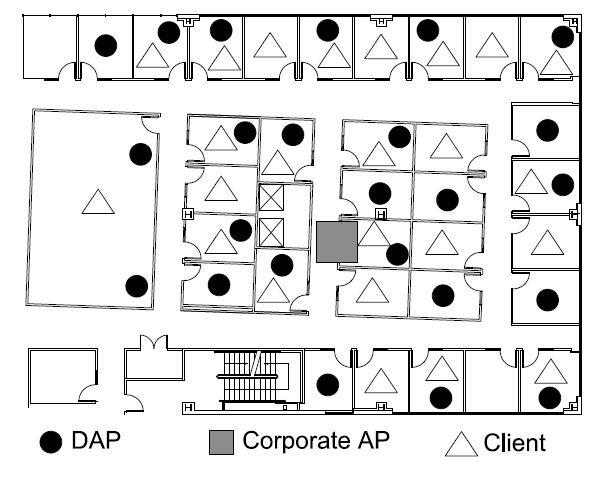
\includegraphics[scale=0.27]{img/fig6.png}
  \end{column}
  \end{columns}
\end{frame}

\begin{frame}{Performanța DenseAP în 802.11g}
  CTS-to-self nu a fost implementat pentru DAP
  \begin{columns}
  \begin{column}{0.5\linewidth}
    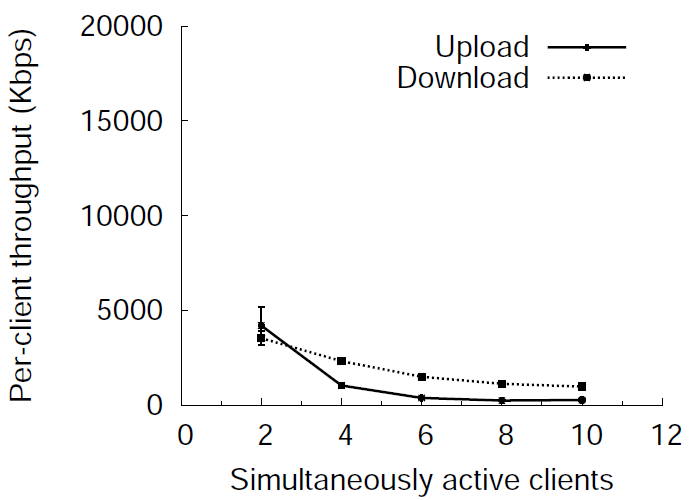
\includegraphics[scale=0.22]{img/fig9.png}
  \end{column}
  \begin{column}{0.5\linewidth}
    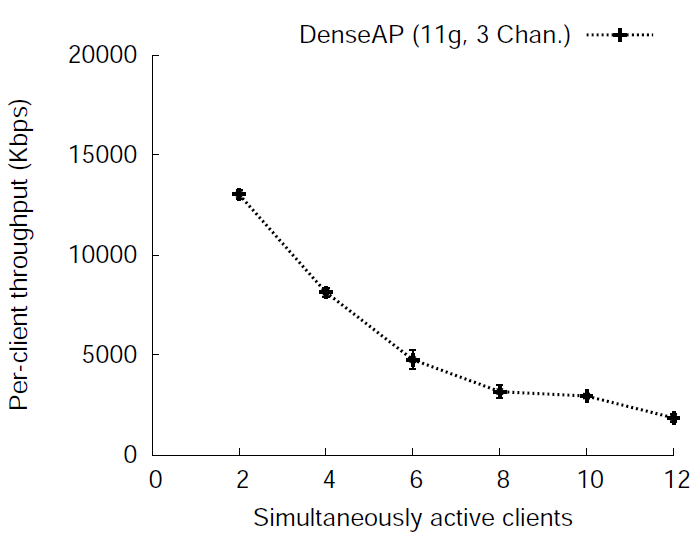
\includegraphics[scale=0.23]{img/fig11.png}
  \end{column}
  \end{columns}
\end{frame}

\begin{frame}{Performanța DenseAP în 802.11a}
  \begin{columns}
  \begin{column}{0.45\linewidth}
    Factori:
    \begin{itemize}
      \item Canale ortogonale
      \item Număr mare de AP-uri
      \item Politica de asociere
      \item Load balancing
    \end{itemize}
  \end{column}
  \begin{column}{0.55\linewidth}
    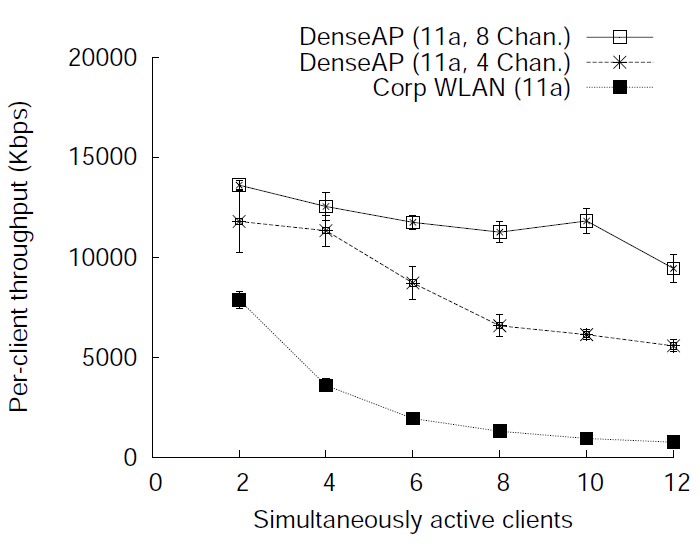
\includegraphics[scale=0.25]{img/fig10.png}
  \end{column}
  \end{columns}
\end{frame}

\begin{frame}{Izolare impact densitate DAP-uri}
  Pentru izolare: DenseAP cu 1 canal
  \begin{center}
    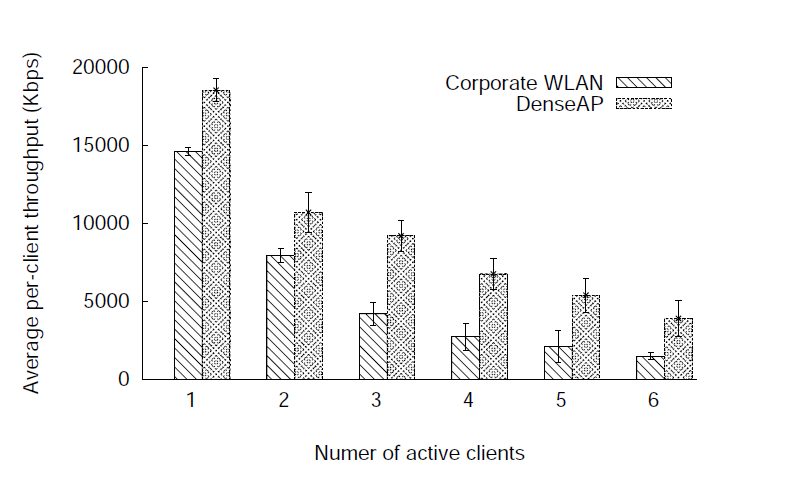
\includegraphics[scale=0.4]{img/fig12.png}
  \end{center}
\end{frame}

\begin{frame}{Izolare impact politica de asociere}
  Asignare canale conform DenseAP, DAP-uri fără ACL
  \begin{center}
    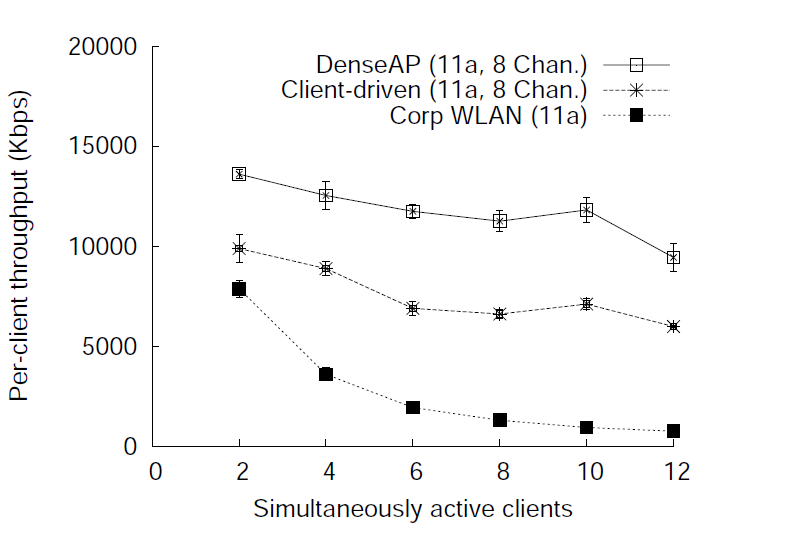
\includegraphics[scale=0.21]{img/fig13.png}
    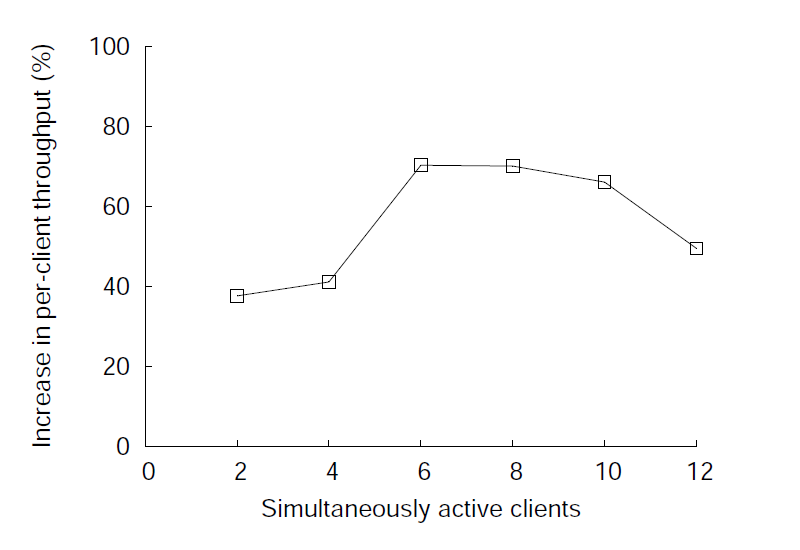
\includegraphics[scale=0.21]{img/fig14.png}
  \end{center}
\end{frame}

\begin{frame}{Performanță cu mai puține DAP-uri}
  \begin{center}
    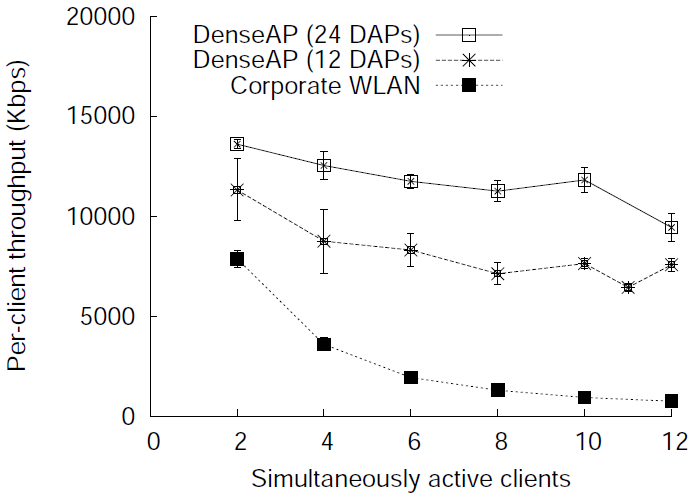
\includegraphics[scale=0.35]{img/fig16.png}
  \end{center}
\end{frame}

\begin{frame}{Performanță cu mai mulți clienți}
  \begin{center}
    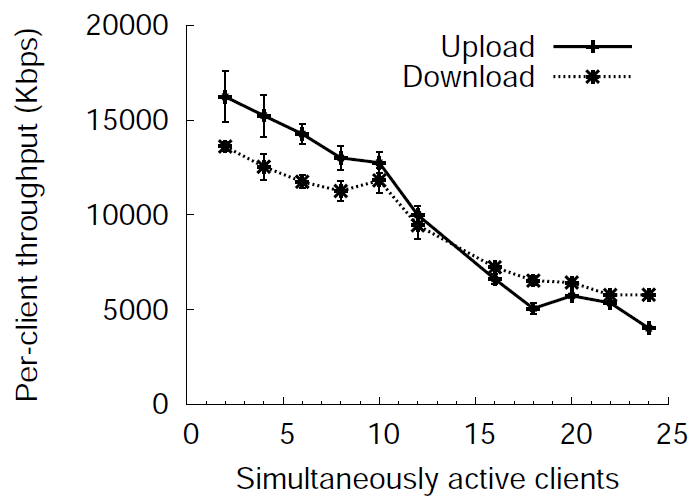
\includegraphics[scale=0.35]{img/fig17.png}
  \end{center}
\end{frame}

\begin{frame}{Trafic sporadic}
  \begin{itemize}
    \item 2000 de fișiere: dimensiunea medie 125KB
    \item Variat timpul între descărcări succesive
  \end{itemize}
  \begin{center}
    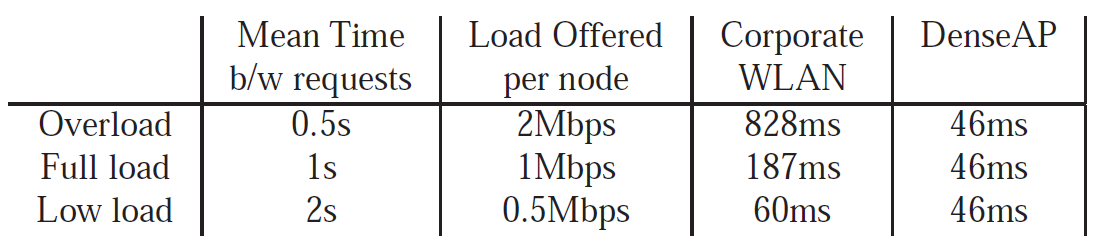
\includegraphics[scale=0.2]{img/table1.png}
  \end{center}
\end{frame}

\begin{frame}{Load Balancing}
  Detectare AP supraîncărcat, migrarea clienților
  \begin{center}
    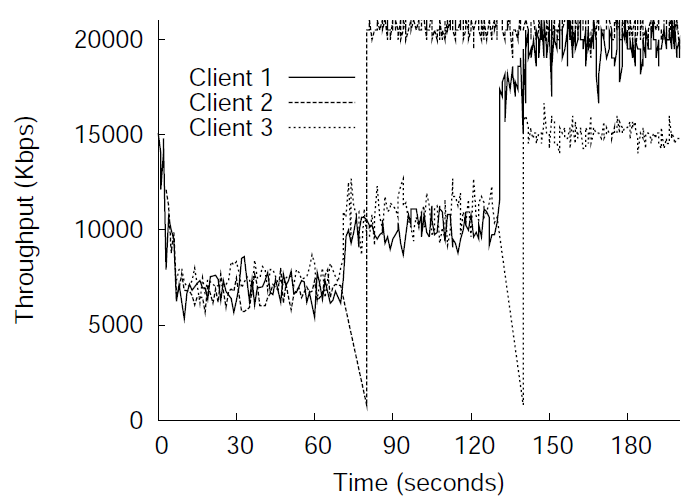
\includegraphics[scale=0.35]{img/fig18.png}
  \end{center}
\end{frame}

\begin{frame}{Handoff}
  \begin{itemize}
    \item Important pentru load balancing și clienți mobili
    \item Posibil TCP timeout din cauza timpului mare de handoff
    \item Clienții trebuie mutați de pe un AP pe altul cât mai rar
  \end{itemize}
  \begin{center}
    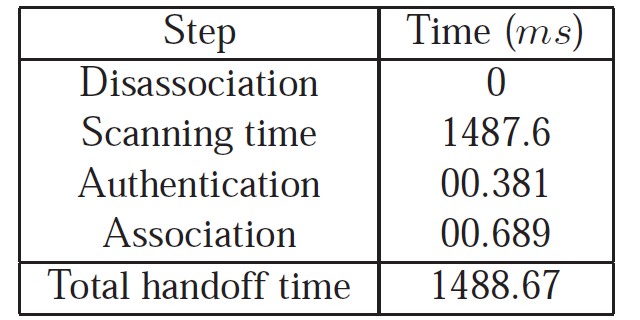
\includegraphics[scale=0.2]{img/table2.png}
  \end{center}
\end{frame}

\begin{frame}{Experimente mobilitate}
  Două tipuri de clienți:
  \begin{itemize}
    \item Nomadic
    \begin{itemize}
      \item schimbă locul, dar petrec perioade semificative de timp în acel loc
    \end{itemize}
    \item Mobil
    \begin{itemize}
      \item în continuă mișcare, clienți VoIP
    \end{itemize}
  \end{itemize}
\end{frame}

\begin{frame}{Performanța DenseAP client tip nomadic}
  \begin{columns}
  \begin{column}{0.4\linewidth}
    \begin{itemize}
      \item 10 descărcări prin TCP de 2MB
      \item 2 minute per loc
      \item fără DenseAP, clientul rămâne asociat la AP1
    \end{itemize}
  \end{column}
  \begin{column}{0.6\linewidth}
    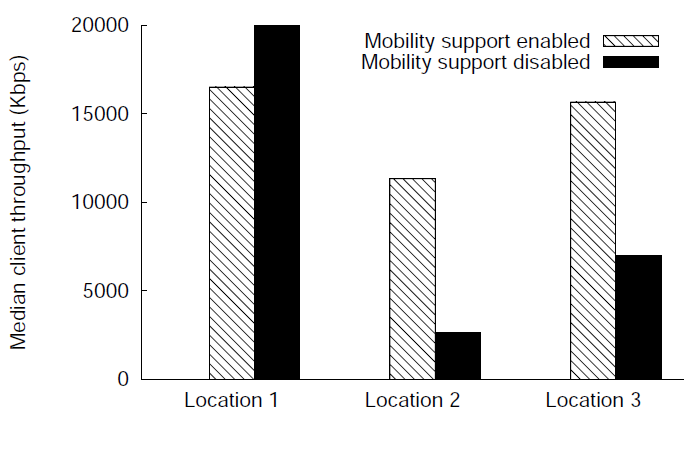
\includegraphics[scale=0.27]{img/fig21.png}
  \end{column}
  \end{columns}
\end{frame}
